\documentclass[a4paper,14pt]{article}

\usepackage{comment} % Para comentar várias linhas ao mesmo tempo

%matemática
\usepackage{amsmath}
\usepackage{amssymb}

%diagramação
\usepackage{extsizes}
\everymath{\displaystyle}
\usepackage{geometry}
\usepackage{fancyhdr}
\usepackage{multicol}
\usepackage{graphicx}
\usepackage[brazil]{babel}
\usepackage[shortlabels]{enumitem}
\usepackage{cancel}
\usepackage{textcomp}
\usepackage{tcolorbox}

%tabelas
\usepackage{array} % Para melhor formatação de tabelas
\usepackage{longtable}
\usepackage{booktabs}  % Para linhas horizontais mais bonitas
\usepackage{float}   % Para usar o modificador [H]
\usepackage{caption} % Para usar legendas em tabelas
\usepackage{wrapfig} % Para usar tabelas e figuras flutuantes


%tikzpicture
\begin{comment}
	\usepackage{tikz}
	\usepackage{scalerel}
	\usepackage{pict2e}
	\usepackage{tkz-euclide}
	\usetikzlibrary{calc}
	\usetikzlibrary{patterns,arrows.meta}
	\usetikzlibrary{shadows}
	\usetikzlibrary{external}
\end{comment}


%pgfplots
\usepackage{pgfplots}
\pgfplotsset{compat=newest}
\usepgfplotslibrary{statistics}
\usepgfplotslibrary{fillbetween}

%colours
\usepackage{xcolor}



\columnsep=2cm
\hoffset=0cm
\textwidth=8cm
\setlength{\columnseprule}{.1pt}
\setlength{\columnsep}{2cm}
\renewcommand{\headrulewidth}{0pt}
\geometry{top=1in, bottom=1in, left=0.7in, right=0.5in}

\pagestyle{fancy}
\fancyhf{}
\fancyfoot[C]{\thepage}

\begin{document}
	
	\noindent\textbf{6FMA08 - Matemática} 
	
	\begin{center}Problemas envolvendo frações (Versão estudante)
	\end{center}
	
	\noindent\textbf{Nome:} \underline{\hspace{10cm}}
	\noindent\textbf{Data:} \underline{\hspace{4cm}}
	
	%\section*{Questões de Matemática}
	
	\begin{multicols}{2}
		\noindent Para calcular a fração $\frac{a}{b}$ de um número $x$, basta fazermos $a \cdot \frac{x}{b}$, ou seja, dividimos $x$ em $b$ partes iguais e tomamos $a$ dessas partes. Por exemplo, para calcular $\frac{3}{5}$ de 30, dividimos 30 em 5 partes iguais (obtendo 6) e multiplicamos por 3, obtendo $3 \cdot 6 = 18$. \\
		Na prática, $\frac{3}{5}$ de 30 é igual a $3 \cdot \frac{30}{5} = 18$. \\
		\noindent\textsubscript{-----------------------------------------------------------------------}
		\begin{enumerate} 
			\item Em uma livraria há 36 livros infantis diferentes. Natália comprou $\frac{1}{9}$ desses livros para seus sobrinhos. Quantos livros ela comprou? \\\\\\\\\\\\\\\\\\\\\\\\\\\\\\\\
			\item O carro da esquerda custa $\frac{1}{4}$ do que custa o carro do meio e este custa $\frac{2}{3}$ do que custa o carro da direita. O carro mais caro custa 630 000 reais. Qual é o preço de cada um dos outros carros? \\ 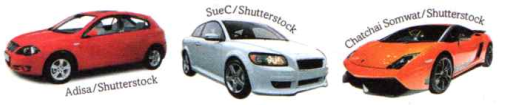
\includegraphics[width=1\linewidth]{6FMA08_imagens/imagem1} \\\\\\\\\\\\\\\\\\\\
			\item \begin{enumerate}[a)]
				\item Carlos tem 4 reais, quantia igual a um terço do que tem seu irmão Manoel. Quanto tem Manoel? \\\\\\\\\\
				\item Caso a quantia que Carlos possui fosse maior, o que ocorreria com a quantia de Manoel? Dê um exemplo. \\
			\end{enumerate}
			\item \begin{enumerate}[a)]
				\item A bilheteria de um teatro vendeu $\frac{1}{6}$ dos ingressos de certa peça. Sabendo que 35 pessoas assistiram a esta peça, calcule o número de assentos disponíveis no teatro. \\\\\\\\\\\\\\\\\\\\\\\\
				\item Complete o enunciado seguindo o modelo do item acima e responda-o: \\
				A bilheteria de um cinema vendeu $\frac{1}{7}$ dos ingressos de certo filme. Sabendo que $\overline{~~~~~~~~~~~}$ pessoas assistiram a esse filme, calcule o número de assentos disponíveis no cinema. \\\\\\\\\\\\\\\\\\\\\\
			\end{enumerate}	
			\item Guilherme viajou de São Paulo ao Rio de Janeiro com seu pai, de carro. Após terem viajado 140 km, pararam para comer alguma coisa. Seu pai lhe disse, então, que haviam andado apenas $\frac{1}{9}$ do caminho. Quantos quilômetros deveriam ainda viajar? \\\\\\\\\\\\\\\\\\\\\\
			%30 a 33
			\item $\frac{1}{8}$ da distância entre São Paulo e Campinas é 12 km. Qual a distância total entre essas duas cidades? \\\\\\\\\\\\\\\\\\\\
			\item Complete:
			\begin{enumerate}[a)]
				\item $3 \cdot \frac{1}{16} = $ .....
				\item $\frac{4}{9} = $ ..... $ \cdot \frac{1}{9}$
				\item $\frac{5}{13} = 5 \cdot $ .....
				\item $\frac{1}{5} + \frac{1}{5} + \frac{1}{5} + \frac{1}{5} = $ ..... $\cdot \frac{1}{5} = $ .....
			\end{enumerate}
			\item \begin{enumerate}[a)]
				\item Mário tem $\frac{1}{4}$ da idade de Luigi. Mário tem 5 anos. Quantos anos tem Luigi? \\\\\\\\\\\\\\\\\\\\\\\\\\
				\item Nesse item, complete o enunciado seguindo o modelo do item acima. Em seguida, resolva-o. Júlio tem $\frac{1}{5}$ da idade de Maria. Júlio tem ..... anos. Quantos anos tem Maria? \\\\\\\\\\\\\\\\\\\\\\\\\\
			\end{enumerate}
			\item \begin{enumerate}[a)]
				\item Manoel comprou 27 bolinhas de gude, mas perdeu $\frac{1}{3}$ delas. Quantas lhe restaram?  \\\\\\\\\\\\\\\\\\\\
				\item Nesse item, complete o enunciado com algum número da tabela abaixo. Em seguida, resolva-o e compare o resultado com o de seus colegas. \\
				Andreia comprou ..... balas, mas deu $\frac{1}{4}$ delas para seu irmão. Quantas lhe restaram? \\
				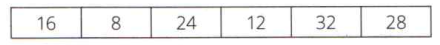
\includegraphics[width=1\linewidth]{6FMA08_imagens/imagem2}
			\end{enumerate}
		\end{enumerate}
		$~$ \\ $~$ \\ $~$ \\ $~$ \\ $~$ \\ $~$ \\ $~$ \\ $~$ \\ $~$ \\ $~$ \\ $~$ \\ $~$ \\ $~$ \\ $~$ \\ $~$ \\ $~$
	\end{multicols}
\end{document}